\documentclass[a4paper,onecolumn,oneside,12pt,extrafontsizes]{memoir}

\usepackage[utf8]{inputenc} % jeśli kodowanie edytowanych plików to UTF8
\usepackage[T1]{fontenc}
\usepackage[polish]{babel}
%\DisemulatePackage{setspace}
\usepackage{setspace}
\usepackage{tabularx}
\usepackage{color,calc}
%\usepackage{soul} % pakiet z komendami do podkreślania tekstu

\usepackage{ebgaramond} % pakiet z czcionkami garamond, potrzebny tylko do strony tytułowej, musi wystąpić przed pakietem tgtermes


\usepackage{tgtermes}   
\renewcommand*\ttdefault{txtt}

\usepackage{listings}

\clubpenalty=10000      %kara za sierotki
\widowpenalty=10000  % nie pozostawiaj wdów
\brokenpenalty=10000		% nie dziel wyrazów między stronami
\exhyphenpenalty=999999		% nie dziel słów z myślnikiem
\righthyphenmin=3			% dziel minimum 3 litery

%\tolerance=4500
%\pretolerance=250
%\hfuzz=1.5pt
%\hbadness=1450

\renewcommand{\topfraction}{0.95}
\renewcommand{\bottomfraction}{0.95}
\renewcommand{\textfraction}{0.05}
\renewcommand{\floatpagefraction}{0.35}

%%%%%%%%%%%%%%%%%%%%%%%%%%%%%%%%%%%%%%%%%%%%%%%%%%%
%%  Ustawienia rozmiarów: tekstu, nagłówka i stopki, marginesów
%%  dla dokumentów klasy memoir 
%%%%%%%%%%%%%%%%%%%%%%%%%%%%%%%%%%%%%%%%%%%%%%%%%%%
\setlength{\headsep}{10pt} 
\setlength{\headheight}{13.6pt} % wartość baselineskip dla czcionki 11pt tj. \small wynosi 13.6pt
\setlength{\footskip}{\headsep+\headheight}
\setlength{\uppermargin}{\headheight+\headsep+1cm}
\setlength{\textheight}{\paperheight-\uppermargin-\footskip-1.5cm}
\setlength{\textwidth}{\paperwidth-5cm}
\setlength{\spinemargin}{2.5cm}
\setlength{\foremargin}{2.5cm}
\setlength{\marginparsep}{2mm}
\setlength{\marginparwidth}{2.3mm}
%\settrimmedsize{297mm}{210mm}{*}
%\settrims{0mm}{0mm}	
\checkandfixthelayout[fixed] % konieczne, aby się dobrze wszystko poustawiało
%%%%%%%%%%%%%%%%%%%%%%%%%%%%%%%%%%%%%%%%%%%%%%%%
%%  Ustawienia odległości linii, wcięć, odstępów
%%%%%%%%%%%%%%%%%%%%%%%%%%%%%%%%%%%%%%%%%%%%%%%%
\linespread{1}
%\linespread{1.241}
\setlength{\parindent}{14.5pt}

\usepackage{memlays} 

%%%%%%%%%%%%%%%%%%%%%%%%%%%%%%%%%%%%%%%%%%%%%%%%%%%%%%%%%%%%%%%%%%                  
%% Definicje stopek i nagłówków
%%%%%%%%%%%%%%%%%%%%%%%%%%%%%%%%%%%%%%%%%%%%%%%%%%%%%%%%%%%%%%%%%%                  
\addtopsmarks{headings}{%
\nouppercaseheads % added at the beginning
}{%
\createmark{chapter}{both}{shownumber}{}{. \space}
%\createmark{chapter}{left}{shownumber}{}{. \space}
\createmark{section}{right}{shownumber}{}{. \space}
}%use the new settings

\makeatletter
\copypagestyle{outer}{headings}
\makeoddhead{outer}{}{}{\small\itshape\rightmark}
\makeevenhead{outer}{\small\itshape\leftmark}{}{}
\makeevenfoot{outer}{\small\thepage}{}{\small\@author:~\@title}
\makeheadrule{outer}{\linewidth}{\normalrulethickness}
\makefootrule{outer}{\linewidth}{\normalrulethickness}{2pt}
\makeatother

%%%%%%%%%%%%%%%%%%%%%%%%%%%%%%%%%%%%%%%%%
%%  Pakiet do generowania indeksu (ważne, aby wstawić przed hyperref)
%%%%%%%%%%%%%%%%%%%%%%%%%%%%%%%%%%%%%%%%%
\DisemulatePackage{imakeidx}
\usepackage[makeindex,noautomatic]{imakeidx} % tutaj mówimy, żeby indeks nie generował się automatycznie, 

%\usepackage[noautomatic]{imakeidx} 
\makeindex

\makeatletter
%%%\renewenvironment{theindex}
							 %%%{\vskip 10pt\@makeschapterhead{\indexname}\vskip -3pt%
								%%%\@mkboth{\MakeUppercase\indexname}%
												%%%{\MakeUppercase\indexname}%
								%%%\vspace{-3.2mm}\parindent\z@%
								%%%\renewcommand\subitem{\par\hangindent 16\p@ \hspace*{0\p@}}%%
								%%%\phantomsection%
								%%%\begin{multicols}{2}
								%%%%\thispagestyle{plain}
								%%%\parindent\z@                
								%%%%\parskip\z@ \@plus .3\p@\relax
								%%%\let\item\@idxitem}
							 %%%{\end{multicols}\clearpage}
%%%
\makeatother

\usepackage{ifpdf}
%\newif\ifpdf \ifx\pdfoutput\undefined
%\pdffalse % we are not running PDFLaTeX
%\else
%\pdfoutput=1 % we are running PDFLaTeX
%\pdftrue \fi
\ifpdf
 \usepackage[pdftex,bookmarks,breaklinks,unicode]{hyperref}
 \usepackage[pdftex]{graphicx}
 \DeclareGraphicsExtensions{.pdf,.jpg,.mps,.png}
\pdfcompresslevel=9
\pdfoutput=1
\makeatletter
\AtBeginDocument{
  \hypersetup{
	pdfinfo={
    Title = {\@title},
    Author = {\@author},
    Subject={},
    Keywords={słowa kluczowe},
  }}
}
\makeatother
\else
\usepackage{graphicx}
\DeclareGraphicsExtensions{.eps,.ps,.jpg,.mps,.png}
\fi
\sloppy

%%%%%%%%%%%%%%%%%%%%%%%%%%%%%%%%%%%%%%%%%
% Metadane dla pdfa

% Deklaracja głębokościu numeracji
\setcounter{secnumdepth}{2}
\setcounter{tocdepth}{2}
\setsecnumdepth{subsection} % activating subsubsec numbering in doc

% Kropki po numerach sekcji
\makeatletter
\def\@seccntformat#1{\csname the#1\endcsname.\quad}
\def\numberline#1{\hb@xt@\@tempdima{#1\if&#1&\else.\fi\hfil}}
\makeatother

\renewcommand{\chapternumberline}[1]{#1.\quad}
\renewcommand{\cftchapterdotsep}{\cftdotsep}

%\definecolor{niceblue}{rgb}{.168,.234,.671}

% Czcionka do podpisów tabel i rysunków
\captionnamefont{\small}
\captiontitlefont{\small}

% Przedefiniowanie etykiet w podpisach tabel i rysunków
%\AtBeginDocument{% 
        \addto\captionspolish{% 
        \renewcommand{\tablename}{Tab.}% 
}%} 

%\AtBeginDocument{% 
%        \addto\captionspolish{% 
%        \renewcommand{\chaptername}{Rozdział}% 
%}} 

%\AtBeginDocument{% 
        \addto\captionspolish{% 
        \renewcommand{\figurename}{Rys.}% 
}%}


%\AtBeginDocument{% 
        \addto\captionspolish{% 
        \renewcommand{\bibname}{Literatura}% 
}%}

%\AtBeginDocument{% 
        \addto\captionspolish{% 
        \renewcommand{\listfigurename}{Spis rysunków}% 
}%}

%\AtBeginDocument{% 
        \addto\captionspolish{% 
        \renewcommand{\listtablename}{Spis tabel}% 
}%}

%\AtBeginDocument{% 
        \addto\captionspolish


%%%%%%%%%%%%%%%%%%%%%%%%%%%%%%%%%%%%%%%
%% Definicja strony tytułowej 
%%%%%%%%%%%%%%%%%%%%%%%%%%%%%%%%%%%%%%%
\makeatletter
%Uczelnia
\newcommand\uczelnia[1]{\renewcommand\@uczelnia{#1}}
\newcommand\@uczelnia{}
%Wydzial
\newcommand\wydzial[1]{\renewcommand\@wydzial{#1}}
\newcommand\@wydzial{}

%Prowadzacy
\newcommand\prowadzacy[1]{\renewcommand\@prowadzacy{#1}}
\newcommand\@prowadzacy{}

%Autorzy
\newcommand\authorOne[1]{\renewcommand\@authorOne{#1}}
\newcommand\@authorOne{}
\newcommand\authorTwo[1]{\renewcommand\@authorTwo{#1}}
\newcommand\@authorTwo{}

\def\maketitle{%
  \pagestyle{empty}%
	\fontfamily{\ebgaramond@family}\selectfont % na stronie tytułowej czcionka garamond

%\setlength{\fboxrule}{\tmpfboxrule} 

	{\centering%\vspace{-1cm}
		{\fontsize{22pt}{24pt}\selectfont \@uczelnia}\\[0.4cm]
		{\fontsize{22pt}{24pt}\selectfont \@wydzial}\\[0.5cm]
		  \hrule \vspace{0.05cm} \hrule 
	}
	
\vspace{2cm}

{\centering
{\fontsize{24pt}{26pt}\selectfont Projektowanie systemów z dostępem w języku naturalnym}\\[2cm]
}


{\centering
{\fontsize{28pt}{30pt}\selectfont \@title}\\[2cm]
}

\begin{center}
\begin{tabular}{ccc}
{\fontsize{16pt}{18pt}\selectfont AUTORZY:}
& 
\hspace{1.5cm}
&
{\fontsize{16pt}{18pt}\selectfont PROWADZĄCY ZAJĘCIA:}
\\ [0.4cm]


{\fontsize{14pt}{16pt}\selectfont \@authorOne}
&
\hspace{1.5cm}
&
{\fontsize{14pt}{16pt}\selectfont \@prowadzacy}
\\ [0.4cm]


{\fontsize{14pt}{16pt}\selectfont \@authorTwo}
&
\hspace{1.5cm}
&

\\ [0.4cm]


\hspace{1.5cm}
&
\hspace{1.5cm}
&
\hspace{1.5cm}
\\ [0.4cm]

\hspace{1.5cm}
&
\hspace{1.5cm}
&
{\fontsize{16pt}{18pt}\selectfont OCENA PRACY:}
\\ [0.4cm]

\end{tabular}
\end{center}


\vspace{7cm}
\hrule\vspace*{0.3cm}
{\centering
{\fontsize{16pt}{18pt}\selectfont \@date}\\[0cm]
}
%\ungaramond
\normalfont
 \cleardoublepage
}



%%%%%%%%%%%%%%%%%%%%%%%%%%%%%%%%%%%%%%%%%
%%  Metadane dokumentu 
%%%%%%%%%%%%%%%%%%%%%%%%%%%%%%%%%%%%%%%%%
\title{Chatbot wspomagający obsługę klienta w sklepie internetowym}
\authorOne{Krystian Lema 218453}
\authorTwo{Bartosz Michalak 218481}
\uczelnia{POLITECHNIKA WROCŁAWSKA}
\wydzial{WYDZIAŁ ELEKTRONIKI}
\prowadzacy{dr inż. Dariusz Banasiak, W4/K9}
\date{WROCŁAW, 2019}


%%%%%%%%%%%%%%%%%%%%%%%%%%%%%%%%%%%%%%%%%
%                  Początek dokumentu 
%%%%%%%%%%%%%%%%%%%%%%%%%%%%%%%%%%%%%%%%%

\begin{document}
\maketitle

\newpage

\chapterstyle{noNumbered}
\pagestyle{outer}
\mbox{}\pdfbookmark[0]{Spis treści}{spisTresci.1}
\tableofcontents*

\newpage

%\include{skroty} %skróty można sobie pominąć
\chapterstyle{default}
\chapter{Wstęp}

\section{Cel projektu}
Celem projektu jest stworzenie chatbota, którego zadaniem jest wsparcie klienta w sklepie internetowym ze sprzętem komputerowym. Komunikacja ma odbywać się w trybie tekstowym. Zadaniem chatbota jest rozpoznanie pytania zadanego przez klienta sklepu internetowego oraz znalezienie odpowiedzi w bazie wiedzy. Wykorzystano również technikę uczenia maszynowego do poprawienia skuteczności chatbota.

\section{Założenia projektowe}
Chatbot ma za zadanie pomagać klientom w następujących tematach:
\begin{itemize}
\item Obsługa konta użytkownika (zmiana hasła, przypomnienie hasła, bezpieczeństwo danych)
\item Dostawa (czas, koszt, rodzaje)
\item Zasady zwrotów (ile czasu na zwrot, koszt zwrotu, sposób)
\item Dostępne metody płatności
\item Śledzenie statusu zamówienia
\item Zasady reklamacji
\item Aktualne promocje
\end{itemize}

\section{Użyte technologie}
Chatbot został napisany w języku programowania Python z użyciem biblioteki dedykowanej do tworzenia chatbotów ChatterBot. ChatterBot to silnik do tworzenia dialogów, który używa bazy wiedzy w postaci plików tekstowych oraz uczenia maszynowego do zwiększenia skuteczności znajdywania odpowiednich odpowiedzi.

\newpage

\section{Zasada działania chatbota}
Schemat działania:
\begin{enumerate}
\item Odczytanie danych
\item Przetwarzanie surowego tekstu
\item Tokenizacja tekstu
\item Usunięcie zbędnych znaków
\item Usunięcie mało znaczących słów
\item Sprowadzenie słów do podstawowych form (lematyzacja)
\item Parsowanie zależności
\item Generowanie odpowiedzi na podstawie bazy wiedzy
\end{enumerate}

\chapter{Implementacja}

\section{Konfiguracja środowiska}
Do stworzenia bota użyto języka Python w wersji 3. W tym celu zainstalowano najnowszą wersję, którą można znaleźć na oficjalnej stronie: \texttt{https://www.python.org/}.
Aby ułatwić pracę w środowisku, dodatkowo zainstalowano managera paczek do Python’a - PIP. Instrukcje dotyczące manualnej instalacji można znaleźć na oficjalnej stronie: \texttt{https://pypi.org/project/pip/}.

\section{Konfiguracja biblioteki ChatterBot}
Instalacja biblioteki ChatterBot jest bardzo prosta przy użyciu PIP. Całą bibliotekę można zainstalować jedną komendą:
\begin{center}
pip install chatterbot
\end{center}
Zainstalowaną bibliotekę można sprawdzić przy pomocy komendy:
\begin{center}
python -m chatterbot --version
\end{center}
Terminal powinien zwrócić aktualną wersję.

\section{Implementacja chatbota}

Pierwszym elementem programu było stworzenie obiektu chatbota. Wykonano to przy pomocy obiektu ChatBot z biblioteki ChatterBot. Podczas tworzenia obiektu chatbota można zainicjalizować go kilkoma parametrami.

\begin{figure}[ht]
	{\centering
		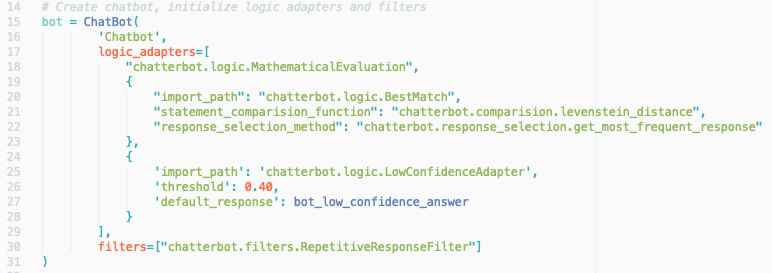
\includegraphics[width=0.9\linewidth]{rys/rys02/1}
	\caption{Tworzenie obiektu bota - kod źródłowy.}
	}
	\label{fig:bot1}
\end{figure}

\newpage

Pierwszym parametrem jest nazwa chatbota.
Kolejnym jest lista adapterów logicznych, których można podać inicjując bota. Nie są one obowiązkowe, ale bez ich określenia, stworzony bot będzie posiadał adaptery domyślne. Aby mieć większą kontrolę nad chatbotem, podano kilka adapterów:
\begin{itemize}
	\item MathematicalEvaluation - dzięki temu adapterowi bot jest w stanie odpowiadać na pytania rozwiązując proste operacje matematyczne. Np. na pytanie $2+2$, powinien zwrócić odpowiedź $4$, która jest prawidłowym wynikiem dodawania.

	\item BestMatch - adapter logiczny, który przy wybieraniu odpowiedzi wybiera tą która najlepiej pasuje do pytania lub po prostu jest tej odpowiedzi najbardziej pewny. Porównywanie odpowiedzi odbywa się przy użyciu algorytmu dogległości Levenstein'a (linia 20 kodu), a z pośród znalezionych odpowiedzi bot wybiera tą, która wystąpiła najczęsciej (linia 21 kodu).

	\item LowConfidenceAdapter - adapter odpowiadający za działanie w przypadku gdy bot nie jest pewny odpowiedzi na zadane pytanie. Adapter ten pozwala ustawić próg poniżej, którego bot nie jest w stanie odpowiedzieć i zwróci tekst informujący o tym np. \textit{Przepraszam ale nie jestem w stanie odpowiedzieć na to pytanie}.
\end{itemize}
Ostatnim parametrem są filtry. Tutaj dodano filtr RepetitiveResponseFilter, który zapobiega powtarzaniu tych samych odpowiedzi przez bota.

\subsection{Uczenie}
Kolejnym etapem jest uczenie bota. Uczenia można dokonać przy pomocy plików tekstowych, zawierających pytania i odpowiedzi w odbpowiednim schemacie. W tym celu stworzono folder, w którym umieszczono wszystkie pliki uczące w formacie \textit{txt}. 

\begin{figure}[ht]
	{\centering
		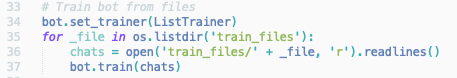
\includegraphics[width=0.7\linewidth]{rys/rys02/2}
	\caption{Uczenie bota - kod źródłowy.}
	}
	\label{fig:bot2}
\end{figure}

Program wczytuje wszystkie pliki w zadanym folderze, otwiera je w trybie odczytu i czyta wszystkie linie. Bot uczy się z każdego pliku, zapamiętuje pytania i odpowiedzi dodając je do bazy danych.

\subsection{Baza wiedzy}
W celu nauczenia bota odpowiedzi na pytania z różnych tematów przygotowano odpowiednie pliki w formacie tekstowym \textit{txt}. Każdy plik odpowiada za inny temat dialogu. Przygotowano odpowiednio dane o tematyce:
\\
\begin{center}
	\begin{tabular}{ll c c}
	- dostawa & 
	- konto klienta \\ [0.3cm]
	
	- płatności & 
	- powitania \\ [0.3cm]
	
	- pożegnania & 
	- promocje \\ [0.3cm]
	
	- reklamy & 
	- zwroty \\ [0.3cm]
	\end{tabular}
\end{center}


Format pliku to pytanie i odpowiedź w kolejnych liniach pliku. 

\begin{figure}[ht]
	{\centering
		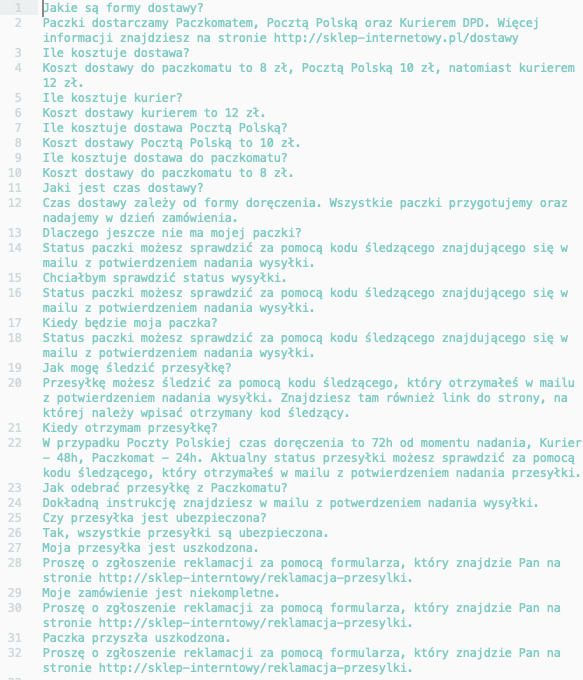
\includegraphics[width=0.9\linewidth]{rys/rys02/3}
	\caption{Przykładowy plik z danymi - dostawa.txt.}
	}
	\label{fig:bot3}
\end{figure}

\newpage


\subsection{Dialog bota z użytkownikiem}

\begin{figure}[ht]
	{\centering
		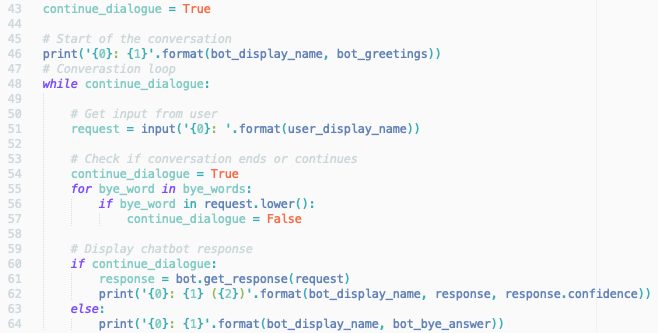
\includegraphics[width=0.9\linewidth]{rys/rys02/4}
	\caption{Dialog bota z użytkownikiem - kod źródłowy.}
	}
	\label{fig:bot4}
\end{figure}

Na samym początku bot zaczyna dialog witając użytkownika i czekając na wprowadzenie tekstu. Dialog zapętlony jest aż do momentu kiedy użytkownik zakończy konwersacje jednym z definiowanych słów pożegnalnych (do widzenia, żegnam, koniec). Po wprowadzeniu tekstu przez użytkownika sprawdzane jest czy nie zakończył on konwersacji. Jeżeli tak, bot żegna się i program kończy działania. W przeciwnym wypadku bot analizuje wprowadzony przez użytkownika tekst i wybiera najlepszą odpowiedź. Gdy pewność odpowiedzi bota jest większa niż przyjęty próg $0.4$, odpowiedź zostaje wyświetlona. Dla ułatwienia testowania, z każdą odpowiedzią bota na końcu wyświetlana jest jego pewność jako wartość z przedziału ${\{0,1\}}$.

\begin{figure}[ht]
	{\centering
		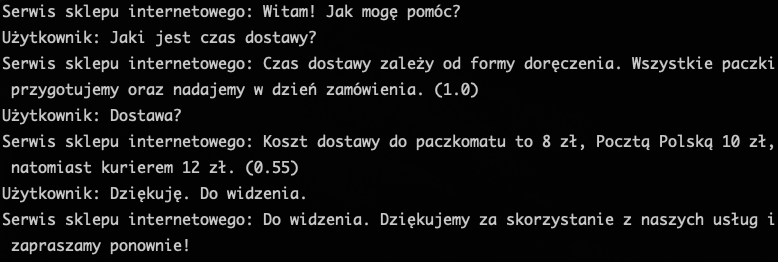
\includegraphics[width=0.9\linewidth]{rys/rys02/5}
	\caption{Przykładowy dialog.}
	}
	\label{fig:bot5}
\end{figure}

\chapter{Testowanie}
\section{Podstawowe testy dialogowe}
\subsection{Powitania}
Jak wspomniano w poprzednim rozdziale, przygotowano zestaw pytań pozwalający na przywitanie się i pożegnanie się przez bota. Przeprowadzono testy sprawdzające, jak reaguje na powitania użytkownika:

\begin{figure}[ht]
	{\centering
		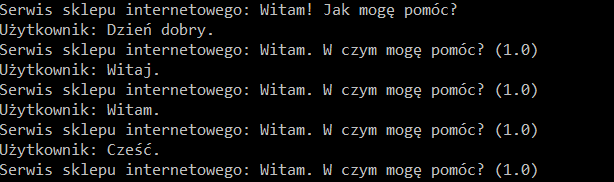
\includegraphics[width=0.9\linewidth]{rys/rys03/1}
	\caption{Reakcja bota na powitania użytkownika.}
	}
	\label{fig:bot4}
\end{figure}

Jak można zaobserwować, pewność odpowiedzi wynosi 100\%. Wynika to z tego, że w bazie wiedzy znajdują się dokładnie te zwroty, których użyto podczas testów.

Kolejnym krokiem było sprawdzenie reakcji na powitania, które zawierają błędy literowe lub zamienioną kolejność wyrazów.

\newpage

\begin{figure}[ht]
	{\centering
		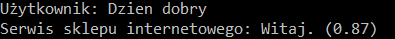
\includegraphics[width=0.9\linewidth]{rys/rys03/2}
	\caption{Reakcja bota na powitanie użytkownika zawierające błąd literowy.}
	}
	\label{fig:bot4}
\end{figure}

Można zaobserwować zmniejszenie pewności odpowiedzi o 13\%.

Kolejnym eksperymentem było sprawdzenie, jak użycie znaków interpunkcyjnych wpływa na pewność odpowiedzi. Wszystkie sekwencje w bazie wiedzy zapisano ze znakami interpunkcyjnymi na końcu zdań oraz pytań. 

\begin{figure}[ht]
	{\centering
		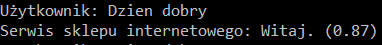
\includegraphics[width=0.9\linewidth]{rys/rys03/3}
	\caption{Powitanie bez znaku interpunkcyjnego na końcu zdania.}
	}
	\label{fig:bot4}
\end{figure}

\begin{figure}[ht]
	{\centering
		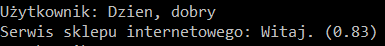
\includegraphics[width=0.9\linewidth]{rys/rys03/4}
	\caption{Powitanie ze znakiem interpunkcyjnym pomiędzy dwoma słowami.}
	}
	\label{fig:bot4}
\end{figure}

Na rysunku 3.3. można zaobserwować obniżenie pewności o 13\%. 
Na rysunku 3.4. widać obniżenie pewności o kolejne 4\% w związku z dodaniem niewystępującego przecinka pomiędzy dwoma wyrazami. 

Wartości te jednak należy uznać za akceptowalne, mając na uwadze, że minimalna pewność odpowiedzi została ustalona na 40\%.

\subsection{Pożegnania}

W bazie wiedzy zawierającej możliwe pożegnania użytkownika zdeklarowano krótkie, w większości składające się z jednego słowa zdania:

\begin{figure}[ht]
	{\centering
		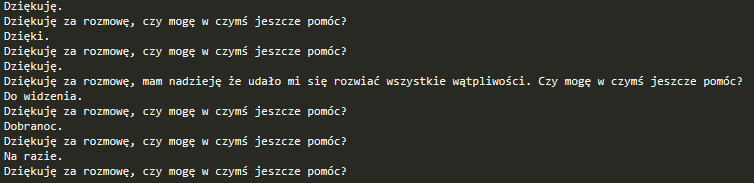
\includegraphics[width=0.9\linewidth]{rys/rys03/6}
	\caption{Baza wiedzy dotycząca pożegnań.}
	}
	\label{fig:bot4}
\end{figure}

Testując interakcję bota w przypadku pożegnania sprawdzono, jak na pewność odpowiedzi wpłynie dodanie dodatkowego słowa do wypopowiedzi użytkownika.

\newpage

\begin{figure}[ht]
	{\centering
		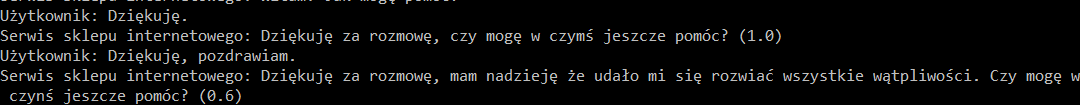
\includegraphics[width=0.9\linewidth]{rys/rys03/5}
	\caption{Pojawienie się dodatkowego słowa w wypowiedzi użytkownika.}
	}
	\label{fig:bot4}
\end{figure}

Na rysunku 3.6. można zaobserwować obniżenie pewności o 40\% w związku z dodaniem jednego słowa do pożegnania.

Kolejnym krokiem było dodanie kolejnego słowa do wypowiedzi użytkownika i sprawdzenie, jak bot poradzi sobie z frazą różniącą się od bazowej o 66\% (3 wyrazy zamiast jednego).

\begin{figure}[ht]
	{\centering
		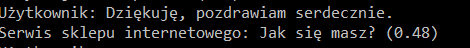
\includegraphics[width=0.9\linewidth]{rys/rys03/7}
	\caption{Pojawienie się dwóch dodatkowych słów w wypowiedzi użytkownika.}
	}
	\label{fig:bot4}
\end{figure}

Zwrócona przez bota nie jest zgodna z oczekiwaną. Współczynnik pewności wynosi 48\% - rozwiązaniem tego problemu mogłoby być m.in.:
\begin{itemize}
	\item
	zwiększenie progu pewności, powyżej którego bot odpowiada na podstawie bazy wiedzy;
	\item
	rozszerzenie bazy wiedzy.
\end{itemize}

\section{Testy zestawów pytań}

Powitania oraz pożegnania to ważna część funkcjonalności bota, jednak nie najważniejsza. Główną funkcjonalność stanowi możliwość pomocy klientowi w podstawych sprawach związanych z zakupami w sklepie internetowym. Kolejnym krokiem było więc przetestowanie wybranych zestawów pytań i odpowiedzi.

\subsection{Pytanie o formę dostawy}

Pierwszym pytaniem, jakie zostało poddane testom, było pytanie o dostępne formy dostawy. W bazie wiedzy zostało ono zapisane w następujący sposób:

\begin{figure}[ht]
	{\centering
		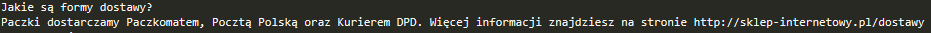
\includegraphics[width=0.9\linewidth]{rys/rys03/8}
	\caption{Pytanie o formy dostawy zapisane w bazie wiedzy.}
	}
	\label{fig:bot4}
\end{figure}

Sprawdzono następujące przypadki:

\begin{itemize}
	\item
	pytanie zgodne w 100\% ze zdefiniowanym w bazie wiedzy.
	\begin{figure}[ht]
	{\centering
		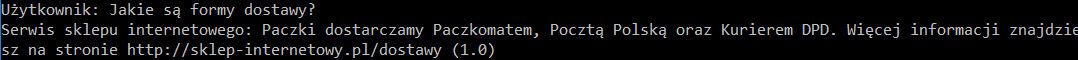
\includegraphics[width=0.9\linewidth]{rys/rys03/9}
	\caption{Odpowiedź bota na pytanie zgodne w 100\% ze zdefiniowanym w bazie wiedzy.}
	}
	\label{fig:bot4}
    \end{figure}
\newpage
	\item
	pytanie bez znaku interpunkcyjnego
		\begin{figure}[ht]
	{\centering
		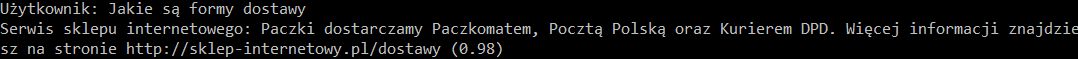
\includegraphics[width=0.9\linewidth]{rys/rys03/10}
	\caption{Odpowiedź bota na pytanie bez znaku interpunkcyjnego.}
	}
	\label{fig:bot4}
    \end{figure}
    
    Warto zwrócić uwagę, że pewność obniżyła się jedynie o 2\%, podczas gdy w przypadku braku znaku interpunkcyjnego dla zdania składającego się z dwóch słów było to 13\%.
	\item
	pytanie zawierające synonim
	\begin{figure}[ht]
	{\centering
		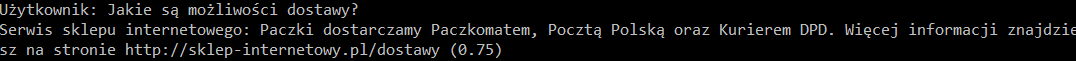
\includegraphics[width=0.9\linewidth]{rys/rys03/11}
	\caption{Odpowiedź bota na pytanie zawierające synonim 'możliwości'.}
	}
	\label{fig:bot4}
    \end{figure}
    
    \begin{figure}[ht]
	{\centering
		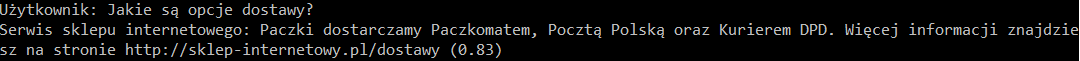
\includegraphics[width=0.9\linewidth]{rys/rys03/12}
	\caption{Odpowiedź bota na pytanie zawierające synonim 'opcje'.}
	}
	\label{fig:bot4}
    \end{figure}
    
    Warto zwrócić uwagę, że pewność boa była inna dla różnych synonimów. Wynika to z liczby znaków poszczególnych synonimów.
	\item
	pytanie zawierające dodatkowe słowo
	
	    \begin{figure}[ht]
	{\centering
		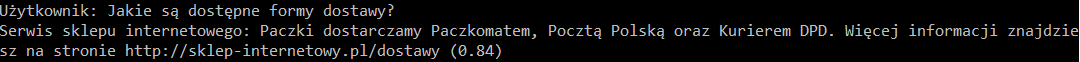
\includegraphics[width=0.9\linewidth]{rys/rys03/13}
	\caption{Odpowiedź bota na pytanie zawierające dodatkowe słowo.}
	}
	\label{fig:bot4}
    \end{figure}
    
    \newpage 
    
	\item
	pytanie zawierające dodatkowe słowo oraz synonim
	
	    \begin{figure}[ht]
	{\centering
		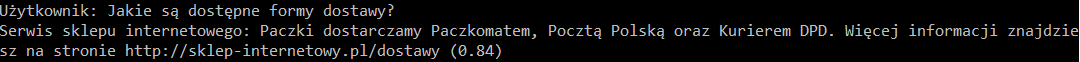
\includegraphics[width=0.9\linewidth]{rys/rys03/13}
	\caption{Odpowiedź bota na pytanie zawierające dodatkowe słowo.}
	}
	\label{fig:bot4}
    \end{figure}
    
\end{itemize}

\subsection{Pytanie o status przesyłki.}

Badany przypadek użycia został w bazie wiedzy zdefiniowany w następujący sposób:

\begin{figure}[ht]
	{\centering
		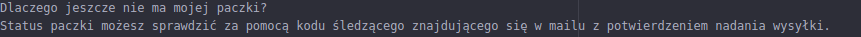
\includegraphics[width=0.9\linewidth]{rys/rys03/15}
	\caption{Definicja pytania w bazie wiedzy}
	}
	\label{fig:bot4}
    \end{figure}

Testom poddano te same sytuacje, co w przypadku poprzedniego pytania. Tym razem jednak badane pytanie zawierało więcej słów.

\begin{itemize}
	\item
	pytanie zgodne w 100\% ze zdefiniowanym w bazie wiedzy.
	\begin{figure}[ht]
	{\centering
		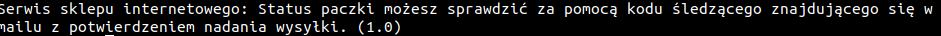
\includegraphics[width=0.9\linewidth]{rys/rys03/16}
	\caption{Odpowiedź bota na pytanie zgodne w 100\% ze zdefiniowanym w bazie wiedzy.}
	}
	\label{fig:bot4}
    \end{figure}

	\item
	pytanie bez znaku interpunkcyjnego
		\begin{figure}[ht]
	{\centering
		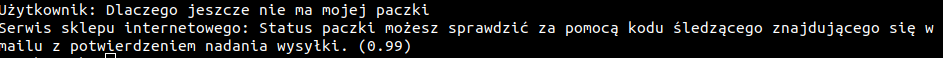
\includegraphics[width=0.9\linewidth]{rys/rys03/17}
	\caption{Odpowiedź bota na pytanie bez znaku interpunkcyjnego.}
	}
	\label{fig:bot4}
    \end{figure}
    
    Po raz kolejny można zaobserwować, że większa liczba słów ma pozytywny wpływ ma pewność odpowiedzi bota w sytuacji pominięcia znaku interpunkcyjnego.
    
    \newpage
    
	\item
	pytanie zawierające synonim
	\begin{figure}[ht]
	{\centering
		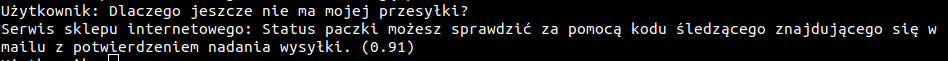
\includegraphics[width=0.9\linewidth]{rys/rys03/18}
	\caption{Odpowiedź bota na pytanie zawierające synonim 'przesyłki'.}
	}
	\label{fig:bot4}
    \end{figure}
    
    
    Pewność bota obniżyła się jedynie o 9\%.
	\item
	pytanie zawierające dodatkowe słowo
	
	    \begin{figure}[ht]
	{\centering
		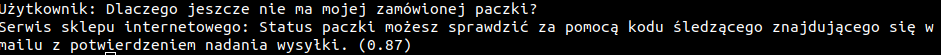
\includegraphics[width=0.9\linewidth]{rys/rys03/19}
	\caption{Odpowiedź bota na pytanie zawierające dodatkowe słowo.}
	}
	\label{fig:bot4}
    \end{figure}
    
    \item
	pytanie zawierające dodatkowe słowo oraz synonim
	
	    \begin{figure}[ht]
	{\centering
		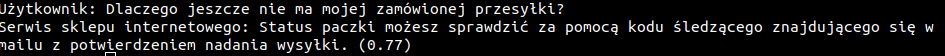
\includegraphics[width=0.9\linewidth]{rys/rys03/20}
	\caption{Odpowiedź bota na pytanie zawierające dodatkowe słowo oraz synonim}
	}
	\label{fig:bot4}
    \end{figure}

\end{itemize}

\newpage
\section{Zwiększanie efektywności bota poprzez zwiększenie bazy wiedzy}


\chapter{Wnioski}

\section{Ogólne wnioski na temat działania chatbota}

\section{Wpływ bazy wiedzy na skuteczność działania}

\renewcommand{\bibname}{Literatura}
\begin{thebibliography}{9}

\bibitem{chatterbot-documentation}
\textit{Dokumentacja ChatterBot'a}
\\\texttt{https://chatterbot.readthedocs.io/en/stable/chatterbot.html}\\dostęp: 08.01.2019

\bibitem{python-documentation}
\textit{Dokumentacja Python'a}
\\\texttt{https://docs.python.org/3/}\\dostęp: 08.01.2019



\end{thebibliography}


 
\end{document}